\section{Network programming}
\label{sec:network-programming}

For the better part of the history of computing, computers have worked
in isolation. Calculations that took place in one computer were
independent from those taking place in another one. The only way that
computers could communicate was by passing programs or data 
indirectly using external data storage units
like perforated tapes, magnetic disks, or CDs (and using a human being
to move them from one computer to the next). 
%
In the 1960s-70s computers were physically huge machines to which
users connected through so-called dumb terminals. In the 1980s-90s
personal computers became the norm, and therefore there were many more
computers in the world, but they were still mostly isolated from each
other.

The development of network technologies and the Internet made it
feasible to communicate computers directly and in real time, faster
and faster every year. This has opened the door to network
programming, where programs run in more than one computer at the same
time. In the early stages, most of the computation was done in one
machine (where the data was) and a little part of it (visualising the
results) was done in another one (where the human user was). Nowadays,
grids and clouds are 
able to run programs on several computers at the same time, each of
them working only on a small part of 
the problem, giving the general impression
of having a bigger, broader, more powerful computer running the whole
program. 

In this section we will learn how to create programs that run in more
than one computer, different objects of the same program communicating
with each other through the network, even if they live on different
machines. Although the topic of network programming is very broad and
exceeds the scope of this module, the main concepts that we
will learn are common to several different technologies. 

\subsection{The basics}
\label{sec:basics}

Most network applications follow the client--server
paradigm\footnote{In recent years, the P2P (peer to peer) model has
  become quite popular. In P2P applications, all computers act as client
  \emph{and} server at the same time.}. This means that the program has two 
parts: \emph{server} and \emph{client}. The former is
runnning in a well-known computer, waiting for clients to request its
services.  \emph{Clients} run on different computers and use the
services provided by the server. Attentive readers may have noticed
that this looks similar to classes calling methods of other classes,
and this is actually the way in which it is modelled in many
object-oriented languages as we will see later.

Depending on the application, the server and the client can be
perceived as the same program or as two different programs. 
For example, web servers (like
Apache) and web browsers (like Mozilla Firefox or Google Chrome) are
seen as different programs, and actually they are developed by
different teams of people. On the other hand, the clients and the
servers of games like World of Warcraft are considered to be part of
the same program. This is only a matter of perception: at a technical
level, client and server are always two different processes with two
different and unrelated memory spaces (stack and heap), usually on two
different machines\footnote{Some applications, including databases and
email programs, have different client and server processes running on
the same machine.}. 

By metonymy, the words client and server are commonly used to refer to
the machines where the server or the clients run. For example,
depending on the context, the term ``web server'' may refer to the
program that serves web pages (like Apache) or a physical computer
where this program is running (like 'www.dcs.bbk.ac.uk'). 

\subsection{Remote Method Invocation (RMI)}
\label{sec:remote-meth-invoc}

There are many technologies to create network applications. Some 
popular ones include RPC, CORBA, RMI, REST, GWT, servlets, and web
services. Most of them have several things in common. We are going to
learn to use RMI (the acronym is for Remote Method Invocation). 

RMI applications are based on the client--server paradigm. Servers are
implemented by objects that expose (i.e.~implement) some
interface. Clients are commonly implemented as objects too. Servers
and clients are usually living on different machines, so clients
cannot execute the methods on the server objects directly; they would
need a pointer to the object, and pointers can only exist inside their
own memory space. 

In order to be able to call methods on objects that do no exist on
their own machine, clients ask the \emph{registry} for a \emph{stub} to the
server. The registry is a special kind of program ---a sort of white
pages--- where servers can register themselves, and then clients can
ask for a reference to a server by providing a name. 
On request, the registry will
provide a reference to a stub for those servers that have been registered. 

\begin{figure}[hbtp]
  \centering
  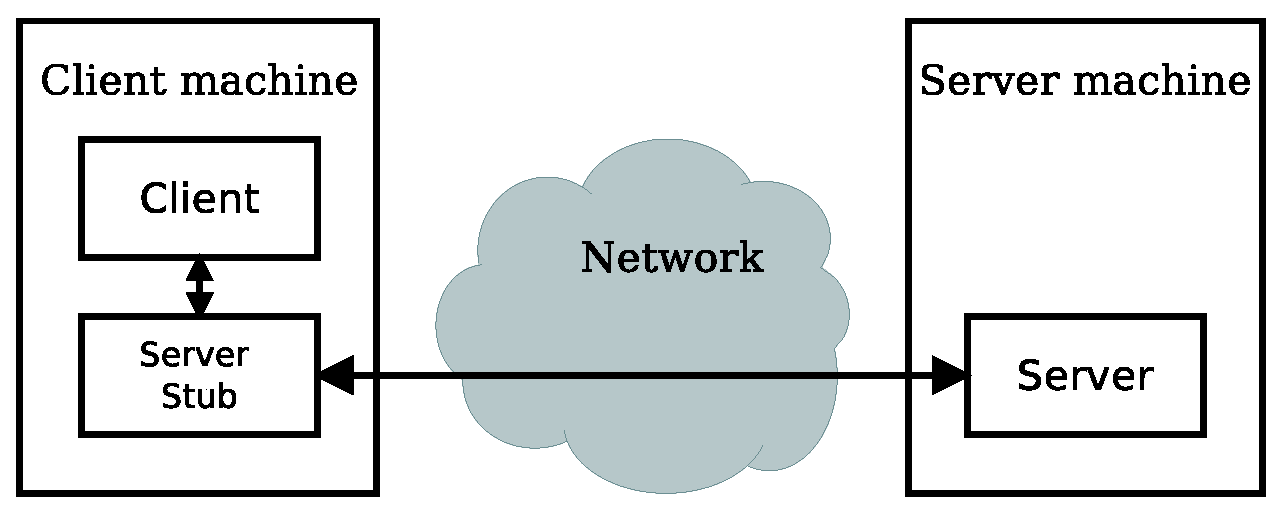
\includegraphics[width=\textwidth]{gfx/rmi-flow}
  \caption{Flow of information (method calls, return values) in RMI}
  \label{fig:rmiflow}
\end{figure}

The stub implements the same interface (i.e.~the same methods) as the
server, so the client can call them (Figure~\ref{fig:rmiflow}) directly. 
However, the stub does not do any
real computation: it ``just'' packs up the parameters provided by the client and
sends them to the server through the network. The server receives
those parameters, runs the appropriate code, and returns a result
through the network to the stub. The stub can then return this result
to the client 
(Figures~\ref{fig:rmiflow1},~\ref{fig:rmiflow2},~\ref{fig:rmiflow3}). 
The good thing about RMI is that almost all the
complexity of the network communication (opening up sockets,
serializing objets as parameters, recovering from network errors, etc)
is hidden from the programmer. From the point of view of the programmer, it
looks (almost) like a normal method call. 

\begin{figure}[hbtp]
  \centering
  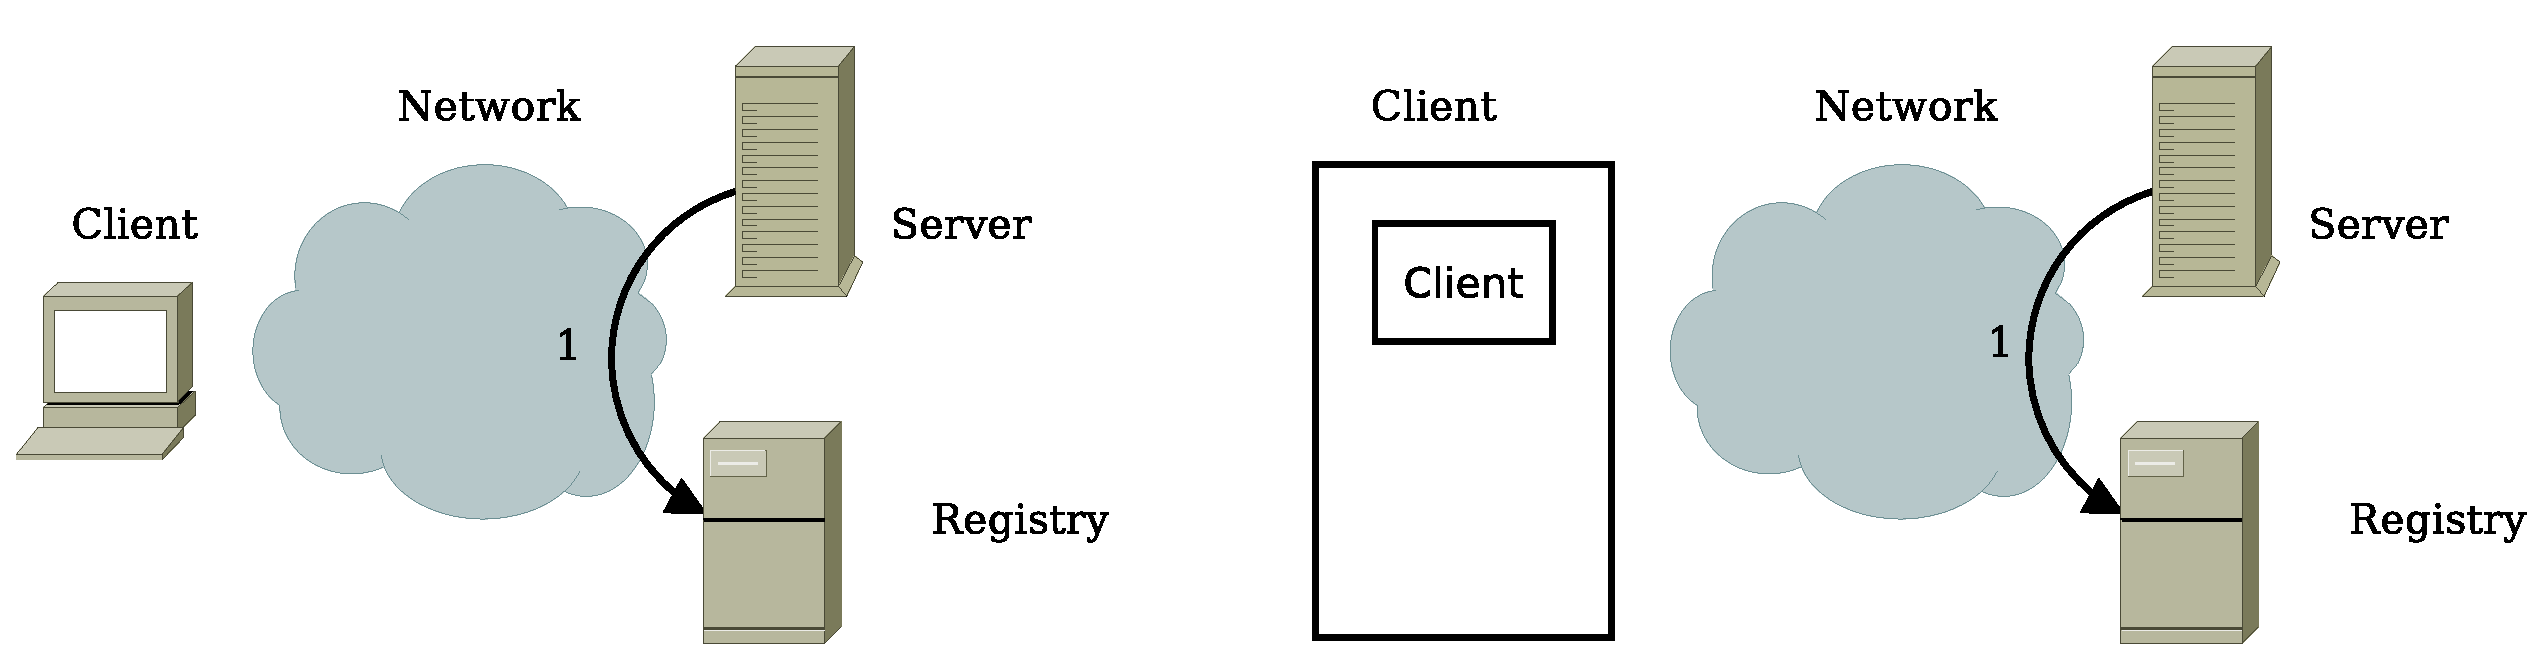
\includegraphics[width=\textwidth]{gfx/rmi-steps1}
  \caption{RMI step by step: (1) the server registers (binds) itself
    on the registry. The server and the registry are very often on the
    same physical machine. }
  \label{fig:rmiflow1}
\end{figure}

\begin{figure}[hbtp]
  \centering
  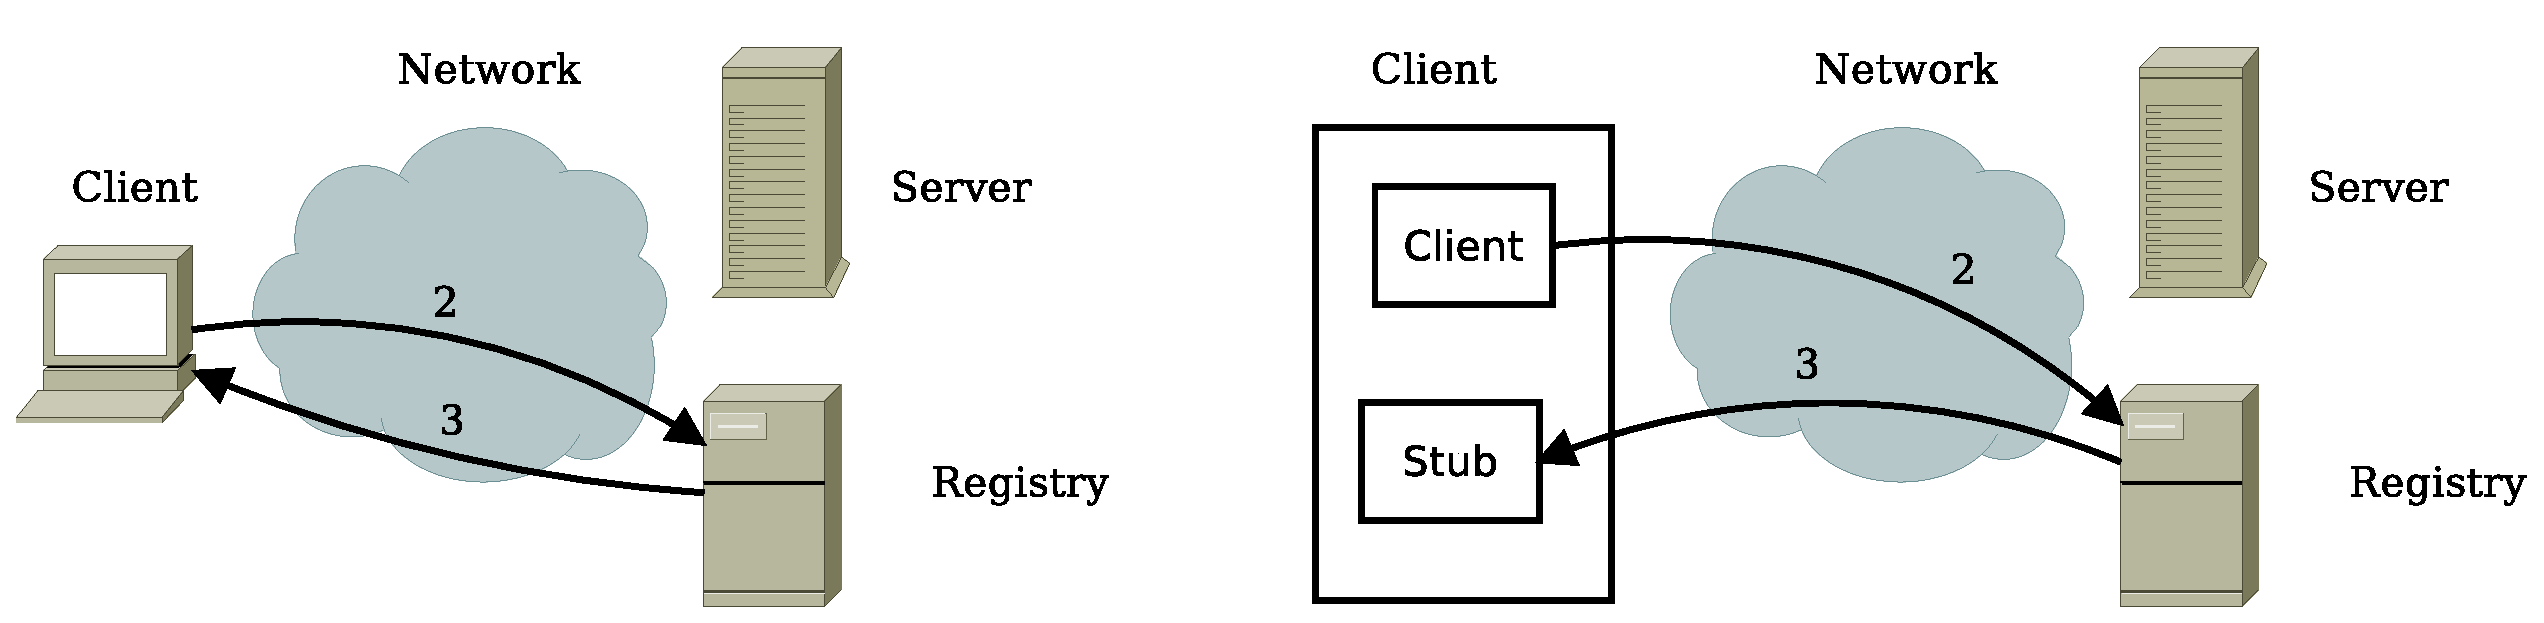
\includegraphics[width=\textwidth]{gfx/rmi-steps2}
  \caption{RMI step by step: (2) the client requests a stub for a
    server (as identified by a name) from the registry, 
    and (3) the registry provides a
    reference to a stub of a server object if it
    has registered with the right name already. }
  \label{fig:rmiflow2}
\end{figure}

\begin{figure}[hbtp]
  \centering
  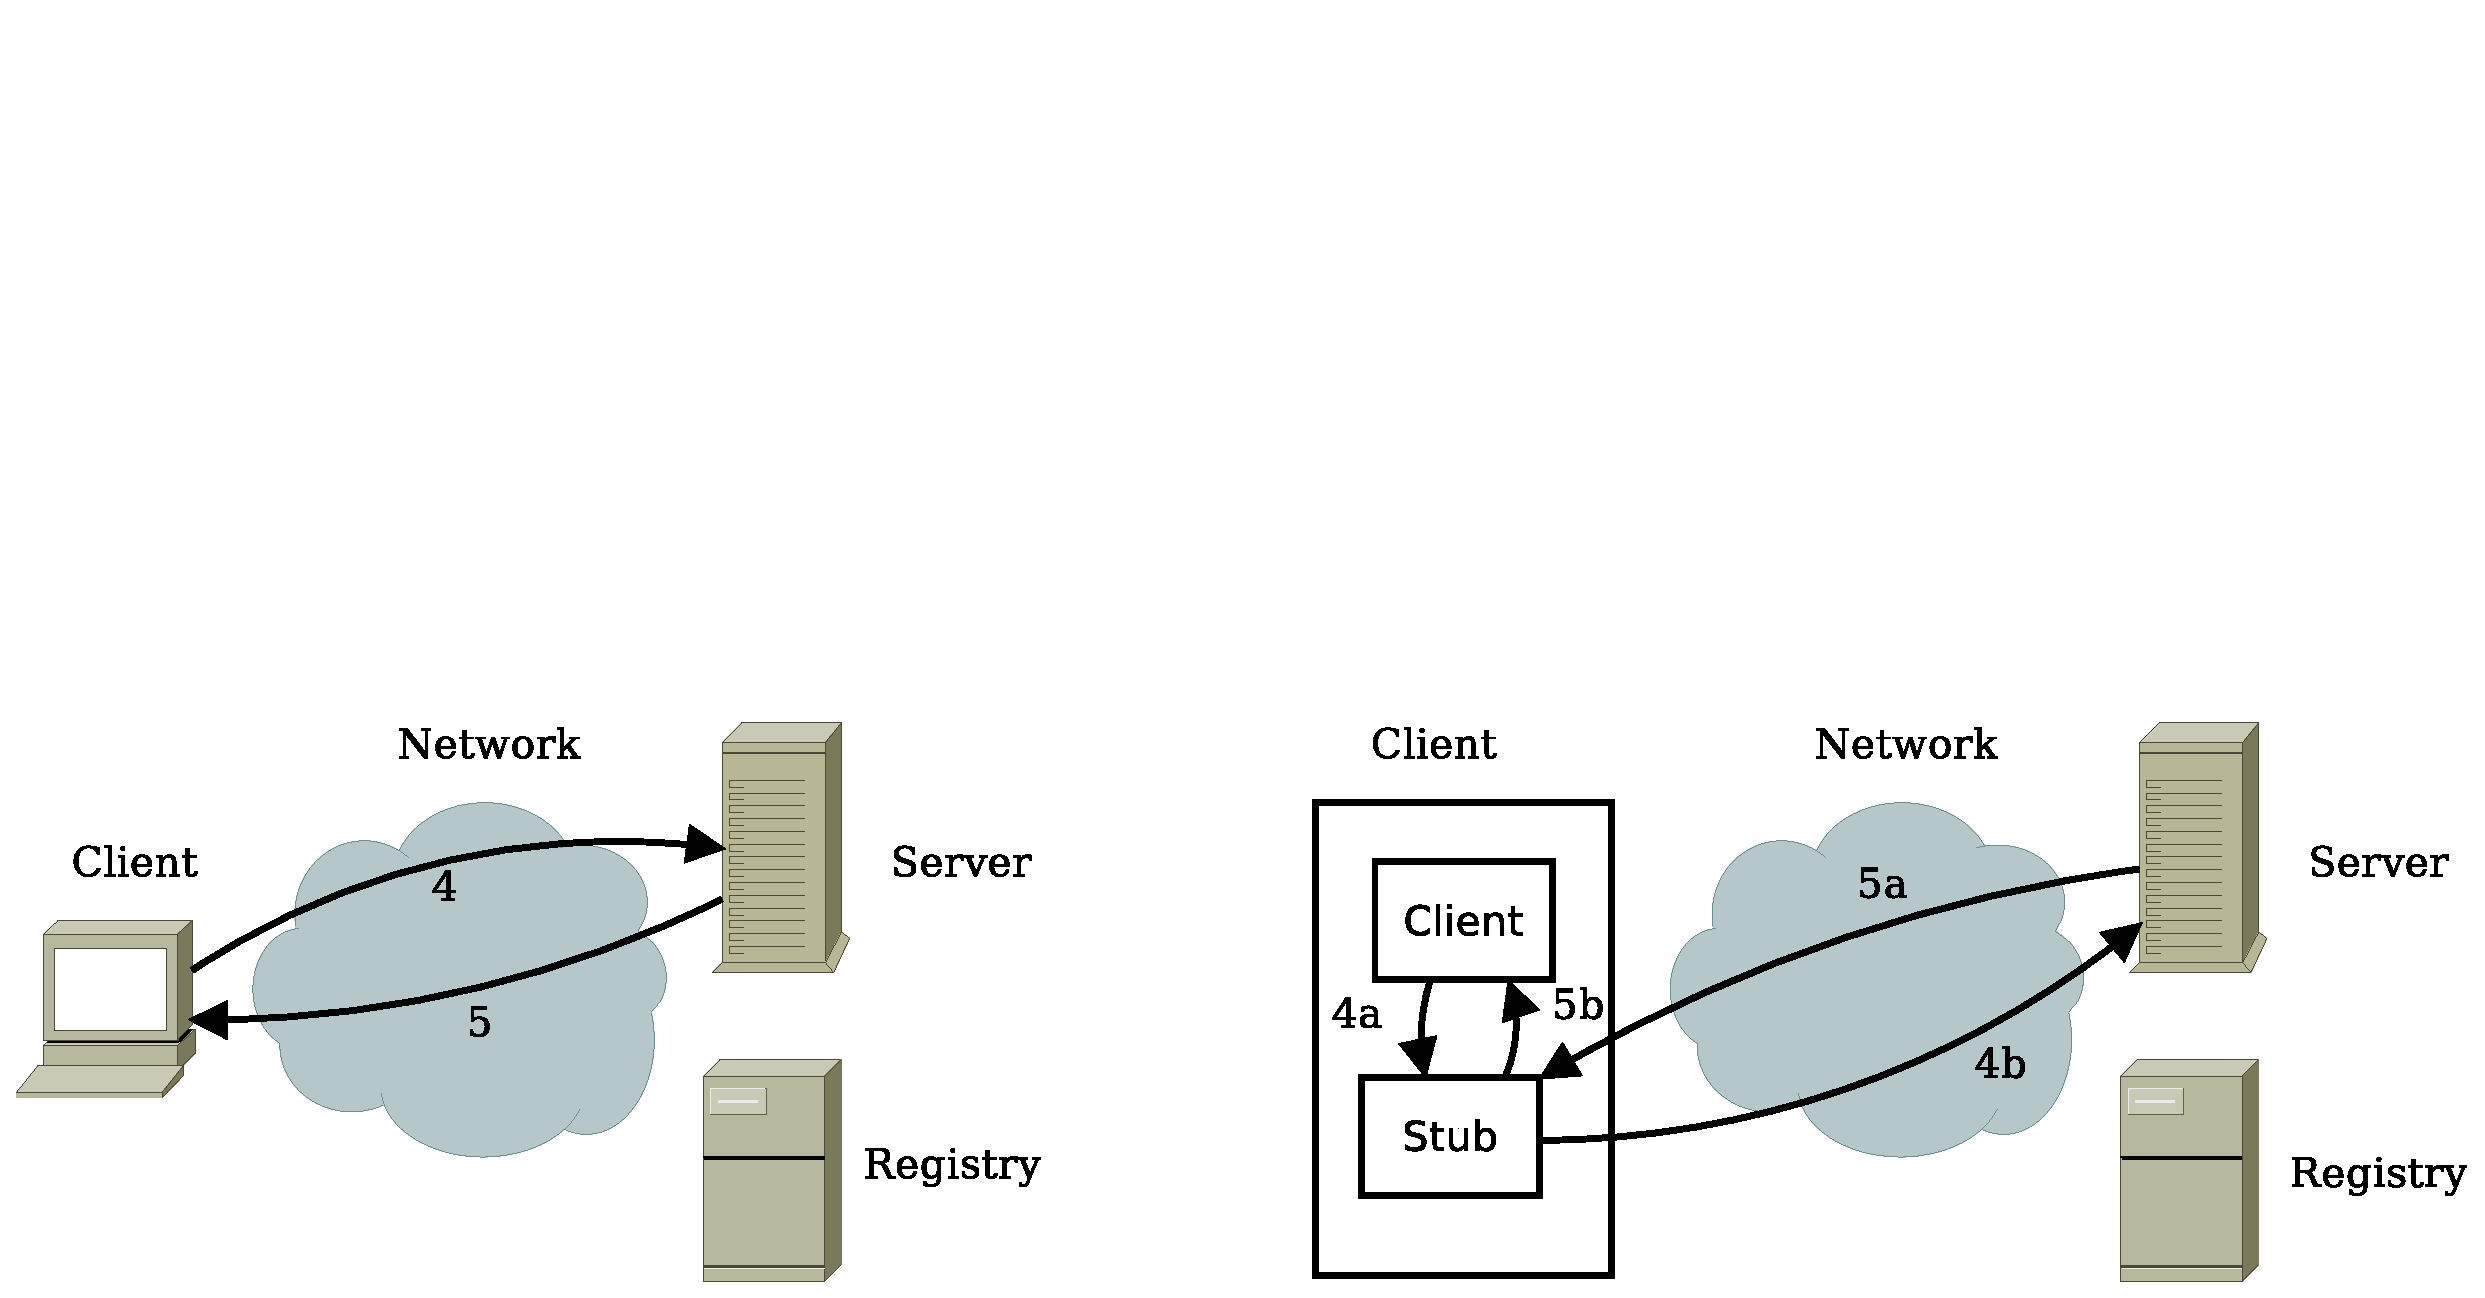
\includegraphics[width=\textwidth]{gfx/rmi-steps3}
  \caption{RMI step by step: (4) the client ---by means of the stub---
  calls a method of the server, and (5) gets a return value. }
  \label{fig:rmiflow3}
\end{figure}

\subsection{Security issues}
\label{sec:security}

When computation is distributed among different machines there are
security concerns to address. Who can access the machine? For what
purpose? 

Security issues are handled in RMI (and Java, in general) by means of security
policies. Although a full revision of security policies in Java goes
beyond of the scope of this section, the basic concepts that we need
for running simple RMI applications are simple to grasp. 

Security policies are defined in text files, usually in the same
folder as the main class is. A basic example of such a file would
have the following aspect: 

\begin{verbatim}
   grant {
     permission java.net.SocketPermission "127.0.0.1:*", "accept,connect";
     permission java.net.SocketPermission "192.168.0.1:80", "connect";
   };
\end{verbatim}

This file would allow code on this machine to accept connections from
machines ``127.0.0.1'' (which
means \emph{localhost}, i.e.~the machine the program is running on) on
any port, and to connect to machine ``127.0.0.1'' on any port or to
machine ``192.168.0.1'' on port 80. 

% TODO: maybe a little more explanation here would be good?

\subsection{Offering a remote service through RMI}
\label{sec:offer-remote-serv}

The first step to offer some service using RMI is to define the
interface of the service. This is a normal Java interface, with two
additional details: it must extend \verb+java.rmi.Remote+, and its
methods must throw \verb+java.rmi.RemoteException+ (in case anything
goes wrong with network connectivity). 

If we had a very simple service called \verb+echo+ that just returned
the same string that was provided as a parameter\footnote{Such a
  service actually exists, and it used to be employed to verify
  network connectivity. A modern parody / homage can be accessed at
  www.ismycomputeron.com.}, 
its interface may look like this: 

\begin{verbatim}
    import java.rmi.Remote;
    import java.rmi.RemoteException;

    /** 
     * An implementation of the echo service.
     */
    public interface EchoService extends Remote {
        /**
         * Returns the same string passed as parameter
         * @param s a string 
         * @return the same string passed as parameter
         */
        public String echo(String s) throws RemoteException;
    }
\end{verbatim}

All objects used as parameters or return values in a RMI interface
must implement the interface \verb+java.io.Serializable+. This is a
tagging interface ---an interface with no methods--- that indicates
that Java should be able to ``flat down'' the object into bytes
(this is called \emph{serializing}) 
and then reconstruct the object again at the other end
(this is called \emph{marshalling}).  
Usual data types from Java (e.g.~Integer, String, etc)
implement \verb+Serializable+.

\subsection{Implementing the service}
\label{sec:implementing-service}

The server that provides the service, 
as we have mentioned, is implemented like a normal Java
object\ldots with two additional details. First, the server object
must extend \verb+UnicastRemoteObject+ (this means that it cannot 
extend another class!). Second, an explicit constructor
must be provided ---even if empty--- that throws
\verb+RemoteException+

The implementation of the interface above could look like (comments
ommitted for brevity): 

\begin{verbatim}
import java.rmi.RemoteException;
import java.rmi.server.UnicastRemoteObject;

public class EchoServer extends UnicastRemoteObject implements EchoService {

    public EchoServer() throws RemoteException {
        // nothing to initialise for this server
    }

    @Override
    public String echo(String s) {
        // This println is not necessary, but helps verifying whether 
        // the server has received the call or not on the remote machine 
        System.out.println("Replied to some client saying '" + s + "'");
        return s;
    }
}
\end{verbatim}

We can now compile the server and create the stub to be sent to
clients. Compiling the server requires a normal Java compilation: 

\begin{verbatim}
    javac EchoServer.java
\end{verbatim}

This will produce an \verb+EchoServer.class+ file, as we know. To
create the stub, we must use the RMI compiler \verb+rmic+ 
on the class file (not the source file):

\begin{verbatim}
    rmic EchoServer
\end{verbatim}

This will produce an \verb+EchoServer_stub.class+ file. We do not need
to do anything special with it apart from generating it. RMI takes
care of sending it to interested clients. 

\subsection{Launching the server}
\label{sec:launching-server}

Launching a server consists of a series of steps that must be followed
in sequence. They are shown in the following code (this may be in a
different class, maybe in a file called \verb+EchoServerLauncher.java+): 

\begin{verbatim}
    private void launch() {
        // 1. If there is no security manager, start one
        if (System.getSecurityManager() == null) {
            System.setSecurityManager(new RMISecurityManager());
        }
        try {
            // 2. Create the registry if there is not one
            LocateRegistry.createRegistry(1099);
            // 3. Create the server object
            EchoServer server = new EchoServer();
            // 4. Register (bind) the server object on the registy. 
            //    The registry may be on a different machine
            String registryHost = "//localhost/";
            String serviceName = "echo";
            Naming.rebind(registryHost + serviceName, server);
        } catch (MalformedURLException ex) {
            ex.printStackTrace();
        } catch (RemoteException ex) {
            ex.printStackTrace();
        }
    }
\end{verbatim}

If the security manager or the registry are not running, they must be
started. The registry will listen on port~1099 by default, but this
can be changed (e.g.~to pass through a firewall that forbids use of
port~1099). Then an instance of the server class is created and
registered (i.e.~bound) with a given name. This name must be known by
clients that want to use the services offered by the server.

The server can be launched by specifying the security policy (i.e. a
file like described on Section~\ref{sec:security}) on the
command line: 

\begin{verbatim}
    java -Djava.security.policy=server.policy EchoLauncher
\end{verbatim}

\subsection{Using the services from the client}
\label{sec:using-services-from}

We are almost there. The only piece missing is the client! 

After setting up the security manager (using the same code as the
server), the first thing that the client needs to do is to find a
reference to the remote server object. It can do so by asking the
registry:

\begin{verbatim}
    Remote service = Naming.lookup("//127.0.0.1:1099/echo"); 
    EchoService echoService = (EchoService) service;
\end{verbatim}

Assuming the name is right ---if not, a \verb+MalformedURLException+
will be thrown--- and a server has registered with the right name (in
this case, ``echo'') ---otherwise, the registry will not find it and
will throw a \verb+NotBoundException+---, the registry will return the
stub, which is an object of type \verb+Remote+. In order to use the
methods in interface \verb+EchoService+, the client must downcast it
explicitly to the right type. Once this is done, using the service is
as easy as a normal method call:

\begin{verbatim}
    String receivedEcho = echoService.echo("Hello!");
\end{verbatim}

This simple line will fire steps~4 and~5 
on Figure~\ref{fig:rmiflow}: the stub
will take string ``Hello!'', convert it into bytes, and send them to
the server. The server will reconstruct the string, execute the
method, and send the return value back to the stub. The stub will give
the return value to the client, who will store it in variable
\verb+receivedEcho+. If anything goes wrong at any point, a
\verb+RemoteException+ will be thrown. 

The client can be launched like the server, specifying the security
policy (usually different) on the command line: 

\begin{verbatim}
    java -Djava.security.policy=client.policy EchoClient <someTextHere>
\end{verbatim}

The client must have access (on its CLASSPATH) to the classes needed
to serialize and marshall the objects sent and received to the
server. This includes the stub and those classes used for parameters
and return values. 

\subsection{Summary}
\label{sec:summary}

The steps to be followed on the server side are: 

\begin{enumerate}
\item Define the interface of the service.
\item Implement the service.
\item Compile the server.
\item Compile the stub with \verb+rmic+
\item Write a launcher that binds the server to the registry, and
  execute it. 
\end{enumerate}

The client needs to look up the server at the registry (by providing a
name). Once it has a reference to it (through the stub), it can call
the methods in the interface like it was a local object. 

%%% Local Variables:
%%% mode: latex
%%% TeX-master: "d19"
%%% End:
